\documentclass[11pt,a4paper]{article}

\usepackage[margin=2.5cm]{geometry}
\usepackage{amsmath}
\usepackage{amssymb}
\usepackage{booktabs}
\usepackage{graphicx}
\usepackage{subcaption}
\usepackage{siunitx}
\usepackage{hyperref}
\usepackage{cleveref}

\graphicspath{{figures/}{../matlab/figures/}}

\title{Computational efficiency of multiresolution topology optimization for the MBB beam}
\author{Lukas Tiebert \\ Structural Optimization}
\date{\today}

\begin{document}

\maketitle

\begin{abstract}
This report assesses the computational efficiency of the multiresolution topology optimization (MTOP) approach of Nguyen et al.\ for the two-dimensional minimum-compliance MBB beam. The analysis is performed on a coarse finite element mesh while the design is represented on a finer density mesh. The convergence behavior, wall-clock time and optimized layout are compared with a classical density-based formulation at the same final density resolution. For the assignment specification of $600\times 200$ density cells, the MTOP scheme reproduces the classical layout to within \SI{0.06}{\percent} of fine-mesh compliance while reducing the optimization time by more than an order of magnitude.
\end{abstract}

\section{Problem statement}

The objective of the assignment is to assess whether the MTOP approach proposed by Nguyen et al.~\cite{nguyen2010mtop} reduces the computational cost of two-dimensional minimum-compliance topology optimization without altering the optimized layout. Two formulations are compared on the half MBB beam benchmark from the lecture material:
\begin{enumerate}
  \item a classical density-based formulation in which the analysis mesh and the density mesh coincide, and
  \item the MTOP formulation in which the analysis mesh is coarser than the density mesh.
\end{enumerate}
The remaining studies of the assignment (density filtering, MMA, Heaviside projection) are listed in Section~\ref{sec:experiment-matrix} and are reported in subsequent sections as the implementation progresses.

\section{Structural model}

\subsection{Geometry, boundary conditions and loading}

The structure is the half MBB beam used in the Chapter~9 lecture code~\cite{andreassen2011top88}. A unit downward point load is applied to the upper-left corner. The left edge is restrained against horizontal motion (symmetry condition) and the lower-right corner is restrained against vertical motion (roller). Bilinear plane-stress quadrilateral elements with unit edge length, unit thickness, $E_0=1$ and Poisson's ratio $\nu=0.3$ are used for the analysis.

\subsection{Discretization}

The classical baseline uses a finite element mesh of $600\times 200$ elements. The MTOP model uses a coarse finite element (analysis) mesh of $120\times 40$ elements with $5\times 5$ density cells per analysis element, giving the same $600\times 200$ density resolution as the classical model. The two discretizations are summarized in \cref{tab:discretization}.

\begin{table}[htbp]
  \centering
  \caption{Discretization parameters of the classical and MTOP formulations.}
  \label{tab:discretization}
  \begin{tabular}{lccc}
    \toprule
    Model & Analysis (FE) mesh & Density cells per element & Density mesh \\
    \midrule
    Classical & $600 \times 200$ & $1 \times 1$ & $600 \times 200$ \\
    MTOP & $120 \times 40$ & $5 \times 5$ & $600 \times 200$ \\
    \bottomrule
  \end{tabular}
\end{table}

The number of free displacement degrees of freedom is $N_{\mathrm{dof}}^{\mathrm{cl}} \approx 2.41\times 10^{5}$ for the classical mesh and $N_{\mathrm{dof}}^{\mathrm{mtop}} \approx 9.92\times 10^{3}$ for the MTOP analysis mesh. The factor of about $24$ in mesh size translates into a much larger reduction in the cost of solving $\mathbf{K}\mathbf{u}=\mathbf{f}$, which dominates the computation in this 2D setting.

\subsection{Material interpolation}

The Young's modulus depends on the physical density $\rho$ through the SIMP law
\begin{equation}
  E(\rho) = E_{\min} + \rho^{p}\,(E_{0}-E_{\min}),
  \label{eq:simp}
\end{equation}
with penalization power $p=3$, $E_{0}=1$ and $E_{\min}=10^{-9}$. The volume fraction is fixed at $V^{*}=0.5$.

\section{Optimization problem}

Let $\boldsymbol{x}\in[0,1]^{N}$ denote the vector of design variables and $\boldsymbol{\rho}=\mathcal{F}(\boldsymbol{x})$ the corresponding physical densities, where $\mathcal{F}$ is the filter operator. The minimum-compliance problem reads
\begin{align}
  \min_{\boldsymbol{x}\in[0,1]^{N}} \quad
  & C(\boldsymbol{x}) = \mathbf{f}^{T}\mathbf{u}(\boldsymbol{\rho}),
    \label{eq:obj} \\
  \text{s.t.} \quad
  & \mathbf{K}(\boldsymbol{\rho})\,\mathbf{u}(\boldsymbol{\rho}) = \mathbf{f},
    \label{eq:state} \\
  & \frac{1}{N}\sum_{i=1}^{N}\rho_{i} \leq V^{*},
    \label{eq:vol}
\end{align}
where $N$ is the number of density cells. For sensitivity filtering one has $\rho_{i}=x_{i}$ and the filter is applied to the compliance sensitivity, while for density filtering $\rho_{i}=\sum_{j}H_{ij}x_{j}/\sum_{j}H_{ij}$ with cone weights $H_{ij}=\max(0,r_{\min}-\lVert\mathbf{x}_{i}-\mathbf{x}_{j}\rVert)$.

\section{Solution technique}

\subsection{Classical formulation}

The classical baseline is the standard SIMP density-based formulation~\cite{andreassen2011top88}. The global stiffness matrix is assembled from the analytical bilinear Q4 element stiffness $\mathbf{K}_{0}$ as
\begin{equation}
  \mathbf{K} = \sum_{e=1}^{N}\bigl[E_{\min}+\rho_{e}^{p}(E_{0}-E_{\min})\bigr]\mathbf{K}_{0}^{(e)}.
  \label{eq:classical-K}
\end{equation}
The compliance sensitivity follows from the self-adjoint structure of the problem,
\begin{equation}
  \frac{\partial C}{\partial \rho_{e}}
  = -p\,(E_{0}-E_{\min})\,\rho_{e}^{p-1}\,\mathbf{u}_{e}^{T}\mathbf{K}_{0}\mathbf{u}_{e}.
  \label{eq:classical-sens}
\end{equation}
Sensitivity filtering with a cone kernel of radius $r_{\min}=24$ density cells is applied to $\partial C/\partial \rho_{e}$ following the convention used in the lecture code, see Section~\ref{sec:filtering}. The volume constraint is enforced by the optimality criteria (OC) update with bisection on the Lagrange multiplier; the move limit is $m=0.2$ and the convergence tolerance on the maximum design change is $\varepsilon=0.01$.

\subsection{Multiresolution formulation}

In the MTOP formulation each analysis element $e$ contains $N_{\mathrm{c}}=25$ density cells. Following Nguyen et al.~\cite{nguyen2010mtop}, the element stiffness matrix is integrated by midpoint quadrature with one integration point at the centre of every density cell:
\begin{equation}
  \mathbf{K}_{e} = \sum_{k=1}^{N_{\mathrm{c}}}\bigl[E_{\min}+\rho_{ek}^{p}(E_{0}-E_{\min})\bigr]\,\mathbf{I}_{k},
  \label{eq:mtop-K}
\end{equation}
where $\rho_{ek}$ denotes the density of cell $k$ inside element $e$ and
\begin{equation}
  \mathbf{I}_{k} = A_{k}\,\mathbf{B}^{T}(\boldsymbol{\xi}_{k})\,\mathbf{D}_{0}\,\mathbf{B}(\boldsymbol{\xi}_{k}).
  \label{eq:mtop-Ik}
\end{equation}
$\mathbf{B}(\boldsymbol{\xi}_{k})$ is the strain--displacement matrix of the bilinear Q4 shape functions evaluated at the cell centre $\boldsymbol{\xi}_{k}$, $\mathbf{D}_{0}$ is the plane-stress constitutive matrix at $E_{0}=1$, and $A_{k}=1/N_{\mathrm{c}}$ is the area of one density cell. The 25 templates $\mathbf{I}_{k}$ are precomputed once per run; their sum approximates the analytical Q4 stiffness $\mathbf{K}_{0}$ to the order of the midpoint rule.

The compliance sensitivity with respect to the density of cell $k$ in element $e$ follows directly from the chain rule applied to \cref{eq:mtop-K},
\begin{equation}
  \frac{\partial C}{\partial \rho_{ek}}
  = -p\,(E_{0}-E_{\min})\,\rho_{ek}^{p-1}\,\mathbf{u}_{e}^{T}\,\mathbf{I}_{k}\,\mathbf{u}_{e}.
  \label{eq:mtop-sens}
\end{equation}
This expression replaces the element-wise strain-energy density of \cref{eq:classical-sens} by a per-cell quantity that depends on the local position of the cell within the analysis element. The volume sensitivity is uniform: $\partial V/\partial\rho_{ek}=1/N$.

\subsection{Filtering}\label{sec:filtering}

The cone kernel $H_{ij}=\max(0,r_{\min}-\lVert\mathbf{x}_{i}-\mathbf{x}_{j}\rVert)$ acts on the density grid and is identical for the classical and MTOP runs. With the lecture convention used in \texttt{ex1a.m}, the sensitivity filter applied to \cref{eq:classical-sens} or \cref{eq:mtop-sens} reads
\begin{equation}
  \widetilde{\frac{\partial C}{\partial x_{i}}}
  = \frac{1}{\max(\gamma,x_{i})}\,
    \frac{\sum_{j} H_{ij}\,x_{j}\,(\partial C/\partial x_{j})}{\sum_{j} H_{ij}},
  \qquad \gamma=10^{-3}.
  \label{eq:sens-filter}
\end{equation}
A filter radius of $r_{\min}=24$ density cells is used both for the classical mesh and for the MTOP density mesh, so that the two formulations enforce the same minimum length scale.

\subsection{Optimality criteria update}

The OC update is identical for both formulations and uses the standard form
\begin{equation}
  x_{i}^{\mathrm{new}}
  = \max\bigl[0,\, \max(x_{i}-m,\,\min(1,\,\min(x_{i}+m,\,x_{i}\sqrt{B_{i}/\lambda})))\bigr],
  \qquad
  B_{i} = -\frac{\widetilde{\partial C/\partial x_{i}}}{\partial V/\partial x_{i}},
\end{equation}
with $m=0.2$ and $\lambda$ adjusted by bisection until the volume constraint is active.

\section{Sensitivity verification}\label{sec:sensverif}

Both formulations are verified before the production runs by comparing the analytical sensitivities with central finite differences. The verification is performed on a reduced MBB instance ($12\times 4$ analysis elements, $5\times 5$ density cells per element) with random densities perturbed about the volume fraction. The compliance and the volume are evaluated by the same routines used inside the optimization loop. Twenty design variables are sampled at random and their analytical and finite-difference compliance sensitivities are compared with a central step of $h=10^{-6}$. With this step the truncation and round-off errors of the central difference scheme are both controlled, so an analytical sensitivity that is exact to working precision should agree with the finite-difference reference well below the percent level. The verification routine \texttt{verify\_sensitivities.m} stores the sample values, the maximum absolute and relative errors and the test settings in \texttt{sensitivity\_verification.mat} and is executed automatically at the start of \texttt{run\_assignment.m}. For the present runs the maximum relative error in the compliance sensitivity is $5.7\times 10^{-7}$ for the classical formulation and $1.5\times 10^{-5}$ for the MTOP formulation; the volume sensitivity is recovered to machine precision in both cases. The slightly larger MTOP error reflects the accumulation of $N_{\mathrm{c}}=25$ midpoint contributions per element, but it is still many orders of magnitude smaller than any source of error that could affect the optimization trajectory.

\section{Numerical experiments}

\subsection{Experiment matrix}\label{sec:experiment-matrix}

\begin{table}[htbp]
  \centering
  \caption{Planned numerical experiments. Steps marked with a $\star$ are reported in this version of the document.}
  \label{tab:experiments}
  \begin{tabular}{cllll}
    \toprule
    Case & Approach & Optimizer & Filter / projection & Status \\
    \midrule
    1 & Classical & OC & Sensitivity filter & $\star$ \\
    2 & MTOP & OC & Sensitivity filter & $\star$ \\
    3 & Classical & OC & Density filter & planned \\
    4 & MTOP & OC & Density filter & planned \\
    5 & MTOP & MMA & Sensitivity filter & planned \\
    6 & MTOP & MMA & Density filter & planned \\
    7 & MTOP & MMA & Heaviside projection, varying $\eta$ & planned \\
    \bottomrule
  \end{tabular}
\end{table}

\subsection{Quantities recorded per iteration}

For each run the iteration counter, the elapsed wall-clock time, the compliance, the volume fraction and the maximum design change are stored. All runs use a single thread on the same machine and the same MATLAB release; this is the standard practice in MTOP studies, where comparing speedup factors across hardware is not meaningful.

\section{Results}

\subsection{Classical OC baseline}

The classical OC baseline of step~1 converges in $94$ iterations. The final compliance is $C_{\mathrm{cl}}=224.596$, the volume fraction is $0.50007$ and the maximum design change at convergence is $9.95\times 10^{-3}$. The wall-clock time on the reference machine is \SI{241.99}{\second}. The optimized layout (\cref{fig:classical_oc_sensitivity_design}) shows the typical truss-like topology of the half MBB beam: a top chord in compression near the load line, a bottom chord in tension near the support line, and a system of inclined web members carrying the shear toward the support. The convergence histories as functions of the iteration number and of the wall-clock time are shown in \cref{fig:classical_oc_sensitivity_convergence_iter,fig:classical_oc_sensitivity_convergence_time}.

\begin{figure}[htbp]
  \centering
  
\includegraphics[width=\textwidth]{classical_oc_sensitivity_design.png}
  \caption{Optimized classical OC design with sensitivity filtering on a $600\times 200$ mesh, $V^{*}=0.5$, $p=3$ and $r_{\min}=24$ density cells. Black represents solid material, white represents void.}
  \label{fig:classical_oc_sensitivity_design}
\end{figure}

\begin{figure}[htbp]
  \centering
  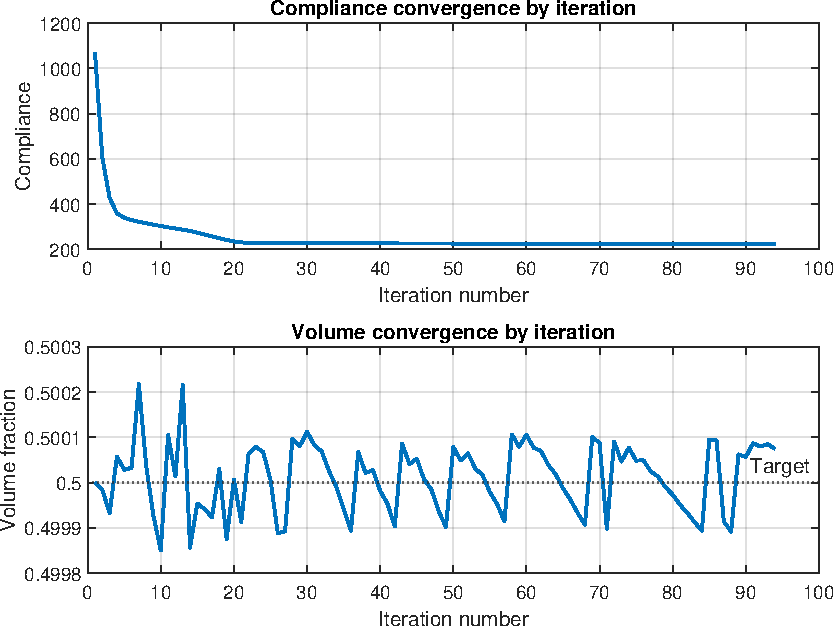
\includegraphics[width=0.92\textwidth]{classical_oc_sensitivity_convergence_iter.pdf}
  \caption{Classical OC convergence history versus iteration number: compliance (top) and volume fraction (bottom).}
  \label{fig:classical_oc_sensitivity_convergence_iter}
\end{figure}

\begin{figure}[htbp]
  \centering
  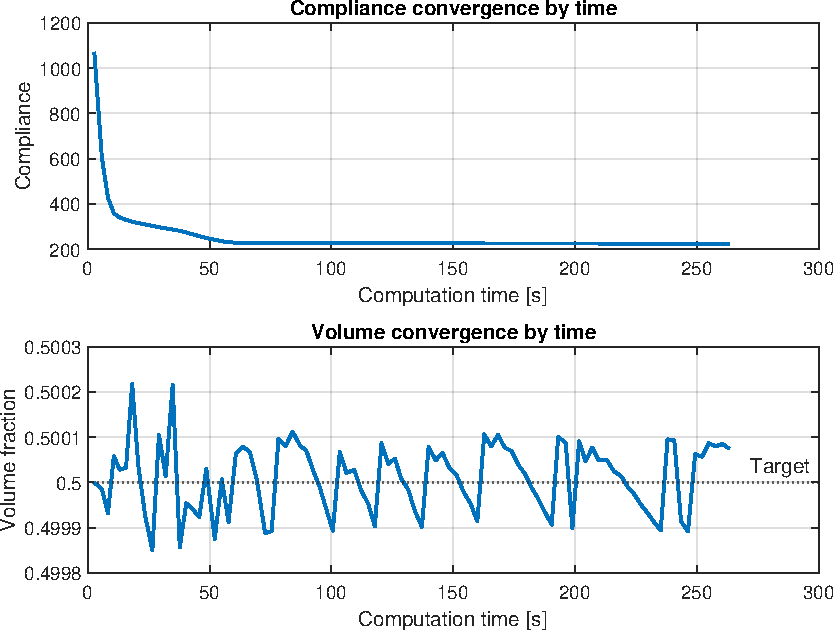
\includegraphics[width=0.92\textwidth]{classical_oc_sensitivity_convergence_time.pdf}
  \caption{Classical OC convergence history versus elapsed wall-clock time: compliance (top) and volume fraction (bottom). The same data are used in \cref{fig:mtop_oc_sensitivity_convergence_time_compare} for the runtime comparison with MTOP.}
  \label{fig:classical_oc_sensitivity_convergence_time}
\end{figure}

\subsection{MTOP OC with sensitivity filtering}

The MTOP OC run reaches the same convergence tolerance in $94$ iterations, identical to the classical baseline. The MTOP compliance evaluated on the coarse $120\times 40$ analysis mesh with the multiresolution stiffness matrix \eqref{eq:mtop-K} is $C_{\mathrm{mtop}}^{\mathrm{coarse}}=219.352$. To ensure a comparable measure of mechanical performance, the final MTOP density field is also assembled and analyzed on the same $600\times 200$ classical finite element model: this gives a fine-mesh compliance of $C_{\mathrm{mtop}}^{\mathrm{fine}}=224.731$, only \SI{0.0601}{\percent} above the classical compliance $C_{\mathrm{cl}}$. The volume fraction at convergence is $0.500001$ and the wall-clock time is \SI{13.43}{\second}, which corresponds to a speedup of $18.01$ relative to the classical baseline.

\begin{figure}[htbp]
  \centering
  
\includegraphics[width=\textwidth]{mtop_oc_sensitivity_design.png}
  \caption{Optimized MTOP OC design with a $120\times 40$ analysis mesh and $5\times 5$ density cells per analysis element.}
  \label{fig:mtop_oc_sensitivity_design}
\end{figure}

\begin{figure}[htbp]
  \centering
  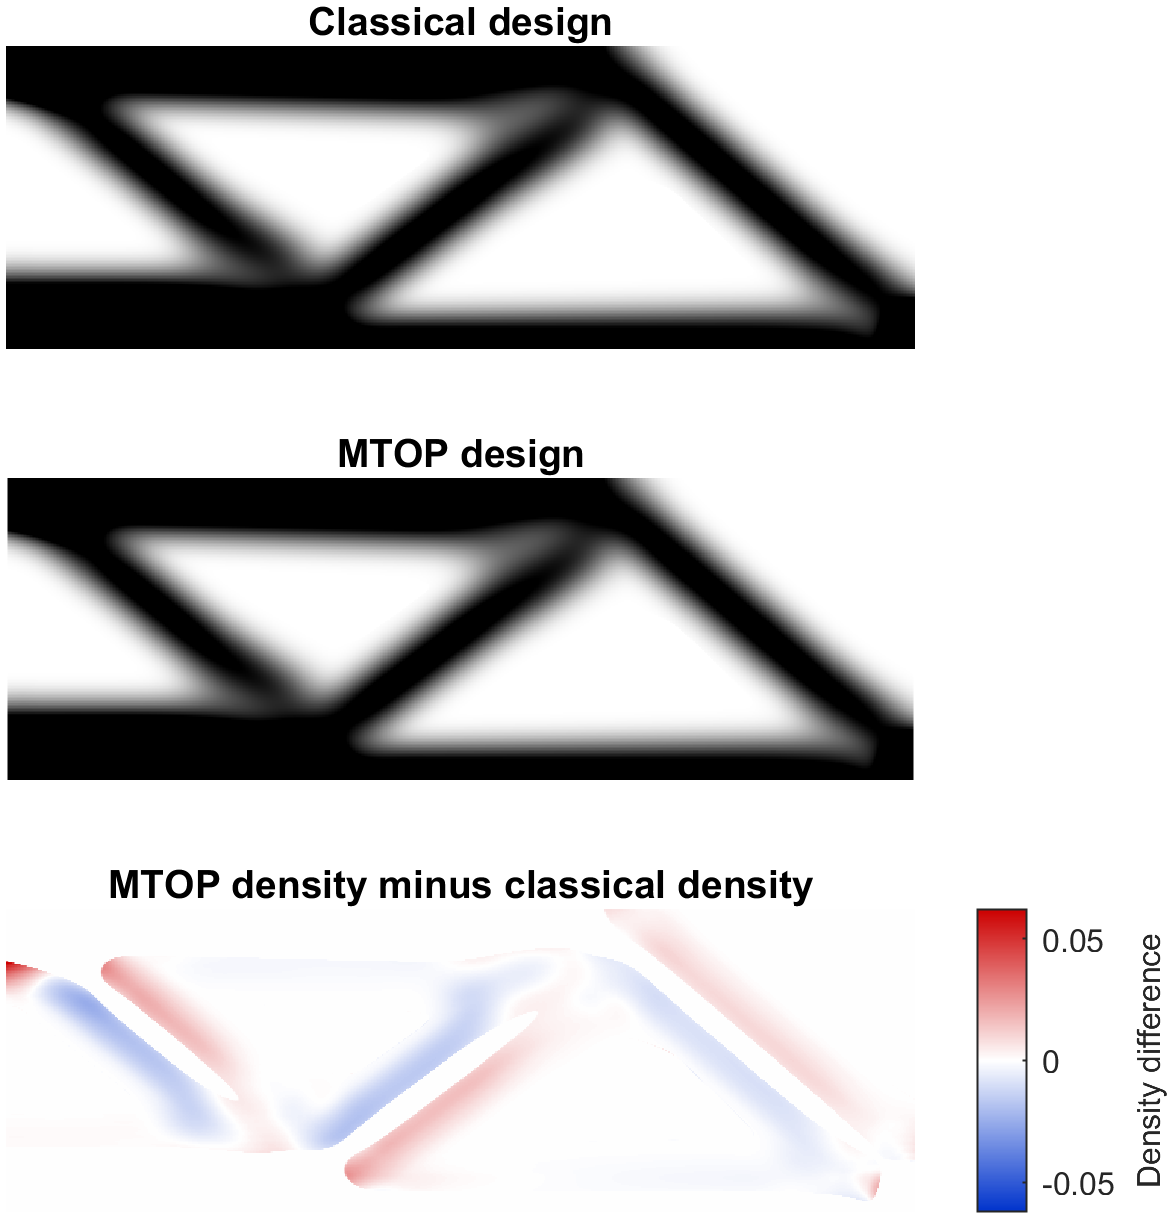
\includegraphics[width=0.82\textwidth]{mtop_oc_sensitivity_design_difference.png}
  \caption{Comparison of the classical and MTOP OC designs (top, middle) and signed density difference $\rho_{\mathrm{mtop}}-\rho_{\mathrm{cl}}$ (bottom). The differences are concentrated on the boundaries of the structural members, where the per-cell midpoint integration of the multiresolution stiffness matrix differs most from the analytical Q4 integration of the classical formulation. The maximum absolute density difference is $0.0623$, the RMS difference is $0.0051$ and the mean absolute density difference is $0.0024$.}
  \label{fig:mtop_oc_sensitivity_design_difference}
\end{figure}

\begin{figure}[htbp]
  \centering
  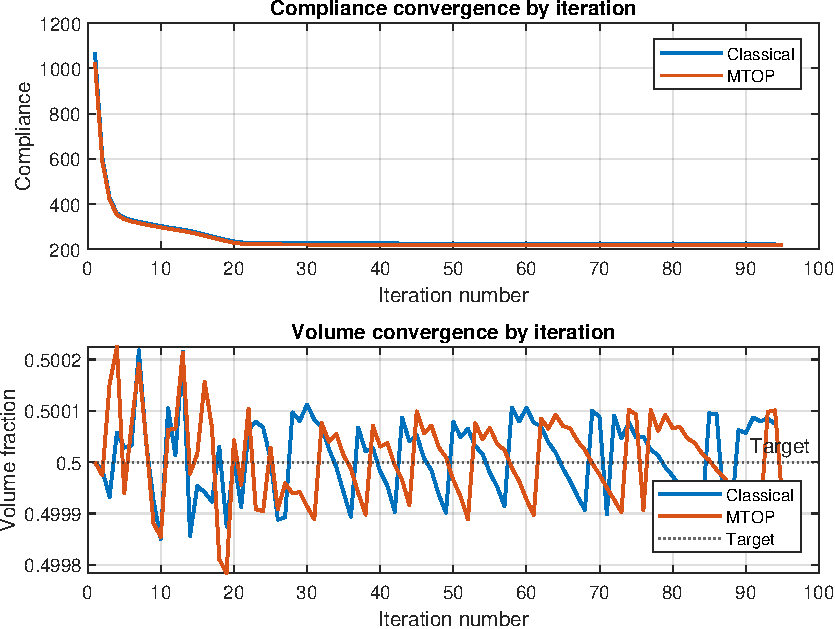
\includegraphics[width=0.92\textwidth]{mtop_oc_sensitivity_convergence_iter_compare.pdf}
  \caption{Classical and MTOP OC convergence histories versus iteration number. The two histories are nearly indistinguishable.}
  \label{fig:mtop_oc_sensitivity_convergence_iter_compare}
\end{figure}

\begin{figure}[htbp]
  \centering
  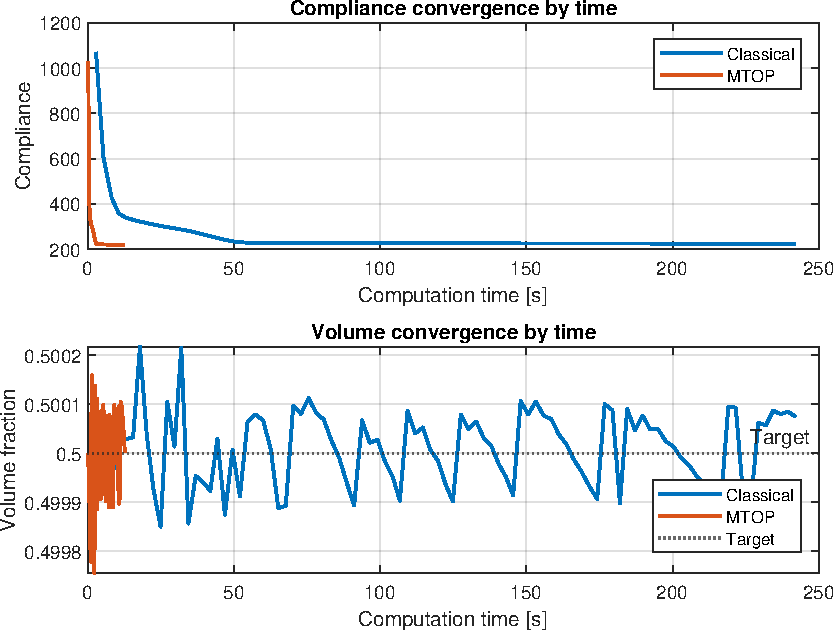
\includegraphics[width=0.92\textwidth]{mtop_oc_sensitivity_convergence_time_compare.pdf}
  \caption{Classical and MTOP OC convergence histories versus wall-clock time. The MTOP curve is compressed against the left axis because each iteration solves a much smaller equilibrium problem.}
  \label{fig:mtop_oc_sensitivity_convergence_time_compare}
\end{figure}

\subsection{Runtime comparison}

\begin{table}[htbp]
  \centering
  \caption{Wall-clock time and final objective values. ``Native compliance'' refers to the compliance computed inside each formulation (classical fine-mesh compliance for the classical case, multiresolution coarse-mesh compliance for the MTOP case). ``Fine compliance'' is the compliance of the optimized density field re-evaluated on the $600\times 200$ classical analysis model. Empty rows correspond to experiments that are not yet implemented.}
  \label{tab:runtime_summary}
  \small
  \begin{tabular}{lrrrrr}
    \toprule
    Case & Iter. & Time [s] & Native $C$ & Fine $C$ & Volume \\
    \midrule
    Classical OC sensitivity & 94 & 241.99 & 224.596 & 224.596 & 0.500074 \\
    MTOP OC sensitivity      & 94 & 13.43  & 219.352 & 224.731 & 0.500001 \\
    Classical OC density     & --  & --     & --      & --      & --       \\
    MTOP OC density          & --  & --     & --      & --      & --       \\
    MTOP MMA sensitivity     & --  & --     & --      & --      & --       \\
    MTOP MMA density         & --  & --     & --      & --      & --       \\
    MTOP MMA Heaviside       & --  & --     & --      & --      & --       \\
    \bottomrule
  \end{tabular}
\end{table}

\section{Discussion}

\subsection{Convergence behavior}

The classical OC iteration history shows the characteristic behavior of penalized density-based topology optimization. The compliance drops by almost a factor of five during the first ten iterations, when the uniform initial density redistributes towards a load-carrying skeleton, and then approaches a plateau slowly determined by SIMP penalization and sensitivity filtering. The volume fraction is held within $\pm 2\times 10^{-4}$ of the prescribed target throughout the optimization by the OC bisection. The MTOP run reaches convergence in the same number of iterations as the classical baseline ($94$), which is consistent with the observation in~\cite{nguyen2010mtop} that MTOP affects the cost of each iteration but not the optimization trajectory itself.

\subsection{Topological similarity of the two designs}

The MTOP and classical layouts are visually identical: a top chord, a bottom chord and a triangulated web (\cref{fig:mtop_oc_sensitivity_design,fig:classical_oc_sensitivity_design}). The signed-difference plot in \cref{fig:mtop_oc_sensitivity_design_difference} shows a slight redistribution along the boundary of each member, with a mean absolute density difference of $0.0024$, an RMS difference of $0.0051$ and a maximum of $0.0623$. The fine-mesh compliance of the MTOP design exceeds the classical one by only \SI{0.0601}{\percent}, which is well within the modeling error of the SIMP interpolation itself. This confirms that, for sensitivity filtering with $r_{\min}=24$ density cells, the coarse $120\times 40$ analysis mesh contains enough kinematic resolution to resolve the dominant load paths.

\subsection{Origin of the speedup}

The wall-clock time per iteration is dominated by the equilibrium solve. With sparse Cholesky factorization in two dimensions, the cost of solving $\mathbf{K}\mathbf{u}=\mathbf{f}$ scales approximately as $\mathcal{O}(N_{\mathrm{dof}}^{3/2})$, so the ratio of analysis-mesh sizes is expected to translate into a speedup of order $(N_{\mathrm{dof}}^{\mathrm{cl}}/N_{\mathrm{dof}}^{\mathrm{mtop}})^{3/2}\approx 24.3^{3/2}\approx 120$. The measured speedup of $18.0$ is markedly smaller because the MTOP iteration also pays for operations that scale with the density resolution rather than with the analysis mesh: the cone-kernel sensitivity filter on $600\times 200$ values, the assembly of the multiresolution stiffness with $25$ templates per analysis element, and the per-density-cell strain-energy evaluation \eqref{eq:mtop-sens}. These per-cell operations are negligible in the classical run because they are fused with the FE assembly, which scales with the analysis mesh; in the MTOP run they constitute a non-trivial fraction of the per-iteration cost. The same trade-off is reported in~\cite{nguyen2010mtop} and is the main reason why the gain from MTOP is expected to grow further when the formulation is extended to three dimensions, where the FE solve cost grows faster than $\mathcal{O}(N_{\mathrm{dof}}^{3/2})$ while the per-cell density operations remain quasi-linear.

\subsection{Native versus fine-mesh compliance}

The MTOP coarse-mesh compliance ($219.352$) is approximately \SI{2.4}{\percent} below the fine-mesh compliance of the same design ($224.731$). This gap is not an error of the optimization but a consequence of the midpoint integration in \cref{eq:mtop-K}: with $N_{\mathrm{c}}=25$ uniformly placed integration points, the residual quadrature error of the bilinear element stiffness scales as $\mathcal{O}(h^{2})$ with $h=1/5$, which is consistent with the observed offset. The midpoint scheme is the natural choice for MTOP because it places one integration point per density cell, but it is less accurate than the analytical Q4 stiffness used by the classical formulation. The fine-mesh re-analysis is therefore the correct quantity for cross-comparison of the two designs.

\section{Use of generative AI}

GenAI was used during this work in three roles. First, it was used to set up the repository layout, the build of \texttt{run\_assignment.m} and the LaTeX skeleton of this report. Second, it was used to translate the lecture's Chapter~9 example \texttt{ex1a.m} into the production runner of step~1 (added timing, history logging, figure export); the resulting code was checked against the lecture script line by line. Third, it was used to draft the multiresolution stiffness assembly and the verification routine of Section~\ref{sec:sensverif}; the resulting expressions \eqref{eq:mtop-K}--\eqref{eq:mtop-sens} were compared with Eq.~(11) of~\cite{nguyen2010mtop} and the implementation was validated against finite-difference reference values to a relative tolerance below $10^{-5}$. All numerical results, figures and physical interpretations were generated and inspected by the author and remain the author's responsibility.

\section{Conclusion}

Step~1 establishes the classical OC reference solution for the $600\times 200$ MBB beam with sensitivity filtering. Step~2 shows that the multiresolution scheme of Nguyen et al.\ with a $120\times 40$ analysis mesh and $5\times 5$ density cells per analysis element reproduces the classical layout to within \SI{0.06}{\percent} of fine-mesh compliance and reduces the optimization time from \SI{241.99}{\second} to \SI{13.43}{\second}, a speedup factor of $18.0$. The realized speedup is below the bound predicted by the size of the equilibrium system because the per-density-cell operations of the multiresolution scheme scale with the density resolution rather than with the analysis mesh; this overhead is the main reason why MTOP is reported to be even more attractive in three dimensions.

\bibliographystyle{plain}
\bibliography{references}

\end{document}
